\documentclass{amsart}
\usepackage{amsmath,amsfonts,amssymb}
\usepackage{tikz-cd}
\usepackage{tikz}
\usepackage{float}
\numberwithin{figure}{section}
\tikzset{
vertex/.style={
draw,
circle,
fill=gray!20,
minimum size=20pt,
inner sep=1pt
}
}
\usepackage{tikz-network}
\usepackage{xkeyval}
\usetikzlibrary{calc}
\title{Brauer Graph Algebras (Schroll)}
\begin{document}
\maketitle
\section{Motivation for Brauer graphs and Brauer graph algebras}

\subsection{Special Biserial Algebras: }

So here, the motivation and idea behind Brauer graphs and Brauer graph algebras is explained.\\

\textbf{(Defn): }Let $K$ be an algebraically closed field. A quiver is a quadruple $Q=(Q_0,Q_1,s,t)$, where \begin{itemize}
    \item $Q_0$ is the set of all vertices 
    \item $Q_1$ is the set of all arrows
    \item A map $s:Q_1 \to Q_0$ which map an arrow $\alpha \in Q_1$ to its starting point $s(\alpha)$ 
    \item A map $t:Q_1 \to Q_0$, which maps the same arrow to its ending point $t(\alpha)$. 
\end{itemize}
In other words, if $\alpha$ is an arrow, then $s(\alpha)$ is the ``head" of the arrow and $t(\alpha)$ is the ``tail" of the arrow. So, a quiver is essentially just a directed graph where loops and parallel arrows are allowed. As such, when we take a loop $\alpha$, then the source and target of the loop is the same. For example, take the following quiver
\begin{figure}[H]
\centering
\begin{tikzcd}[sep=normal]
	&&& 3 \\
	1 && 2 \\
	&&& 4
	\arrow["\mu", from=1-4, to=1-4, loop, in=55, out=125, distance=10mm]
	\arrow["\alpha", from=2-1, to=2-3]
	\arrow["\beta", shift left=2, from=2-3, to=1-4]
	\arrow["\eta"', shift right=2, from=2-3, to=1-4]
	\arrow["\gamma"', shift right=2, from=2-3, to=3-4]
	\arrow["\lambda"', shift right=2, from=3-4, to=2-3]
\end{tikzcd}
\caption{Quiver $Q^{(1)}$}
\label{fig:quiverexample}
\end{figure}

 The above diagram is a quiver where $Q_0=\{1,2,3,4\},Q_1=\{\alpha,\beta,\gamma,\lambda,\mu,\eta\}$. where $s(\alpha)=1$ and $t(\alpha)=2$,$s(\beta)=2=s(\eta)$ and $t(\beta)=3=t(\eta)$, $s(\mu)=t(\mu)=3$, $s(\lambda)=4$ and $t(\lambda)=2$, and $s(\gamma)=2$ and $t(\gamma)=4$\\


 A \textit{path} in $Q$ from a vertex $i$ to another vertex $j$ is a sequence of arrows  $c=(i\mid\alpha_1,\alpha_2,...\alpha_m\mid j)$, where the target of the previous arrow is the source of the next arrow. That is, in $c$, we have $t(\alpha_{k-1})=s(\alpha_k)$ for all $0\leq k \leq t-1$ . Here, we see $s(\alpha_1)=i$ and $t(\alpha_{m})=j$ and we can also denote the start and ending of the paths by $s(p)=\alpha_1$ and $t(p)=\alpha_m$ respectively. The length of the path $c$ is the number of arrows in the path, denoted by $l$ and thus $l(c)=m$. The \textit{lazy} path or trivial path is simply the path $e_i=(i\mid \alpha \mid i)$ for some arrow $\alpha$. In Figure~\ref{fig:quiverexample}, $c_1=(1\mid \alpha,\beta\mid 2)$ is a path. We can also denote paths just by the arrows and dropping the vertices. Then $c_2=\alpha\gamma\lambda$ is also a path from 1 to 2\\
 

 For every quiver $Q$, we can also get its corresponding \textit{path algebra} $KQ$, which is an algebra over the field $K$, and whose underlying vector space is generated by all the paths in the quiver. In other words, the basis of $KQ$ is the set of all paths in $Q$. Also important to note that if the quiver has a loop or an oriented cycle, then there would be infinite paths, and thus the path algebra would be infinite dimensional. The path algebra for the quiver $Q^{(1)}$ in Figure~\ref{fig:quiverexample} is infinite dimensional whereas the path algebra for a quiver with 2 vertices and a single arrow between them would be finite dimensional\\
 
 Like any other algebra (or vector space), the multiplication can be determined by the multiplication of two basis elements. So, here if $c$ and $c'$ are any two basis elements of $KQ$, then the multiplication $c \cdot c'$ is defined by 

 \[
c \cdot c' = 
\begin{cases}c  c' , & \text{if } s(\alpha_k)=t(\alpha_{k-1}) \\
0, & \text{otherwise }
\end{cases}
\]

where $c c'$ is the concatenation of two paths in $Q$(Note that concatenation of two paths is only possible if the ending vertex of $c$ is the starting vertex of $c'$, so that means multiplication in $KQ$ is possible only if concatenation in $Q$ is possible. If it is not we simply define it to be 0). \\


Let us denote by $\mathcal{R}$ the two-sided ideal of $KQ$ generated by all the arrows in $Q$. Another two sided ideal $I$ is called admissible if there exists a positive integer $m\geq 2$ such that 
\[
\mathcal{R}^m \subset I \subset \mathcal{R}^2
\]

Here, $\mathcal{R}^m$ is simply the decomposition $$\mathcal{R}^m=\bigoplus_{l \geq m}KQ_l$$ and as a vector space, it has a basis being the set of all paths greater than or equal to $m$. So, if $I$ is an admissible ideal, then it would contain all the paths greater than or equal to $m$, which would mean that the algebra obtained by quotienting out $I$ from $KQ$, that is, the algebra $KQ/I$ is finite dimensional. We also say that the algebra $KQ/I$ is given by a quiver and relations. The algebra $KQ/I$ is indecomposable if and only if the quiver $Q$ is connected. \\
Also, the condition $I \subset\mathcal{R}^2$ guarantees that when we quotient I out from the path algebra, then we would not cut out any arrows.\\
We need the following definitions for Theorem 1.1: 
\begin{enumerate}
\item \textbf{Connected Algebra: } \textit{Idempotent} elements are those elements $e$ of an algebra $A$ such that $e^2=e$. A \textit{central} idempotent $e$ is an idempotent such that $ea=ae$ $\forall a \in A$. $A$ is called connected if the only central idempotent elements are 0 and 1. In other words, $A$ is connected if $e^2=e\implies e=0$ or 1, with $e$ being a central idempotent.  
\item \textbf{Morita equivalence}: Two algebras $A$ and $A'$ are said to be \textit{Morita equivalent} if their module categories are equivalent. That is, $A$ and $A'$ are Morita equivalent if Mod-$A \simeq$ Mod-$A'$  
\end{enumerate}

 \textbf{Theorem 1.1: } \textit{Every connected finite-dimensional $K$-algebra is Morita equivalent to an algebra $KQ/I$ for a unique quiver $Q$ and where $I$ is an admissible ideal of $KQ$}\\

 
 The above theorem by Gabriel is useful because then we can study arbitrary connected finite-dimensional algebras by studying $KQ/I$ which are more or less well studied(?). This is an especially powerful tool in representation theory of algebras \\

 Nevertheless, algebras of the form $KQ/I$, $I$ being admissible, are still somewhat complicated, and as such, the subclasses of these algebras are considered. So to get these subclasses of these algebras, as an example, we can impose further restrictions on $Q$ and $I$. \\

 An example of such a restriction is on the number of arrows starting and ending at each vertex in the quiver. If at each vertex $v\in Q_0$, there is at most one arrow starting and at most one arrow ending at $v$, then $KQ/I$ is said to be monomial and of \textit{finite representation type}. When we say finite representation type, we mean that the number of isoclasses of the indecomposable distinct $KQ/I$-modules
 An algebra of such type is called as the \textit{Nakayama Algebra}. An algebra $KQ/I$
  is said to be \textit{monomial} if the ideal $I$ is generated by paths. Note that this definition depends on the choice of the ideal $I$. So what this means is that there might be a different ideal $J$(that might not be generated by paths) such that $KQ/I\cong KQ/J$. So this is an open problem/question, raised by Auslander, that is to find a homological characterisation that implies that a given algebra is monomial. This would be a much stronger formulation of a monomial algebra than the one currently given. Even in that case, the current definition still works, and monomial algebras are still well-studied and documented and many open problems have been studied in the case of monomial algebras.\\
  
  After this one, we can explore restrictions that are ``weaker" and thus get a more ``complex" structure. So we have the following:
  \begin{itemize}
      \item[(S0)] For every vertex $i\in Q_0$, there are at most two arrows starting at $i$ and at most two arrows ending at $i$.\\
      While this is a weaker restriction than the previous one, nonetheless it is still a strong restriction on the subclasses of algebras one can consider in general. Most algebras that satisfy this condition (S0) are called algebras of \textit{wild representation type}.

      \item[(S1)] For every arrow $\alpha$ in $Q$, there is at most one arrow $\beta$ such that $\alpha\beta\notin I$ and there exists at most one arrow $\gamma$ such that $\gamma\alpha\notin I$.

      Almost all algebras satisfying condition (S1) (and not necessarily (S0)) are of wild representation type. In fact, algebras satisfying (S1) only are called \textit{special multiserial algebras}
      \end{itemize}
\textbf{Definition 1.2 } A finite-dimensional $K$-algebra $A$ is called special biserial if there exists a quiver $Q$ and an admissible ideal $I$ in $KQ$ such that $A$ is Morita equivalent to $KQ/I$ and such that $KQ/I$ satisfies conditions (S0) and (S1)\\


We now list some important properties and results of special biserial algebras.\\


\textbf{Theorem 1.3} \textit{Special biserial algebras are of tame representation type}\\

\textbf{Definition 1.4: } A finite-dimensional $K$-algebra $A$ is called biserial if every indecomposable projective left and right $A$-module $P$ is such that rad($P)=U+V$ where $U$ and $V$ are uniserial modules and $U \cap V$ is either a simple $A$-module or zero.

So, we define what projective and uniserial modules are. An $R$-module $P$ is said to be \textit{projective} if and only if for every surjective module homomorphism $f : N \to M$ and every module homomorphism $g : P \to M$, there exists a module homomorphism $h : P \to N$ such that $fh = g$.\\
A \textit{uniserial} module $M$ is a module over a ring $R$, whose class of submodules is equipped with a total order defined by inclusion. This means that, if we have any two submodules $N_1$ and $N_2$, we have that either $N_1 \subseteq N_2$ or $N_2 \subseteq N_1$. \\
A \textit{simple} module is a module which has no non-trivial proper submodules\\

\textbf{Theorem 1.5} \textit{Every special biserial algebra is biserial}\\

\textbf{}

\textbf{}
\section{Brauer Graph Algebras}
\textbf{Definition 2.1: } A \textit{Brauer graph} $G$ is a tuple $G=(V,E,m,o)$ where 
\begin{itemize}
    \item $(V,E)$ is an unoriented connected graph with vertex set $V$ and edge set $E$.
    \item $m: V \to \mathbb{Z}^+$ is a function, called the \textit{multiplicity}, which assigns to each vertex a positive integer.
    \item $o$ is called the \textit{orientation} of $G$, and is given as follows: for each vertex $v \in V$, there is a cyclic ordering of the edges incident with $v$. For example, this cyclic ordering may be clockwise or anti-clockwise. If $v$ is incident to only one edge $e$ and $m(v)=1$, then the cyclic ordering is simply given by $e$. If $m(v) > 1$, then the cyclic ordering at $v$ is given by $e<e$.
\end{itemize}

A \textit{Brauer tree} is a Brauer graph $G=(V,E,m,o)$ such that the underlying graph $(V,E)$ is a tree and $m(v)=1$ for all but at most one vertex $v \in V$.\\

From now on, we will also refer to $(V,E)$ simply as $G$ for convenience. In this document, we allow $G$ to have multiple loops and multiple edges.\\

We define the \textit{valency} $\mathrm{val}(v)$ of a vertex $v$ in $G$ to be the number of edges incident with $v$, where loops are counted twice. Equivalently, the valency of $v$ is the number of half-edges incident at $v$, which explains why loops are counted twice.\\

An edge $e$ incident with a vertex $v$ is said to be \textit{truncated} at $v$ if 
\[
m(v)\,\mathrm{val}(v) = 1.
\]

We note that if an edge $e$ is truncated at both of its incident vertices $v$ and $w$, that is, if 
\[
m(v)\,\mathrm{val}(v) = 1 \quad \text{and} \quad m(w)\,\mathrm{val}(w) = 1,
\]
then the Brauer graph $G$ consists of a single edge with both vertices having multiplicity $1$, and the corresponding Brauer graph algebra is $k[x]/(x^2)$.\\

\textbf{Example 2.2: } Let us consider a few examples of Brauer graphs. We will examine the multiplicities and valencies of the vertices, as well as the orientations of the graphs. Here, the orientation is given by locally embedding each vertex of the Brauer graph into the clockwise oriented plane. One could also choose the anti-clockwise orientation, but for now, we will use the clockwise orientation. 

In the following examples, most of the vertices will have multiplicity $1$. If for some $v \in V$ we have $m(v) > 1$, then we will mention the value of $m(v)$  beforehand.
\begin{itemize}
    \item[1)]  Let us take the following Brauer graph $G_1=(V_1,E_1,m_1,o_1)$, where the $V_1,E_1$ are the set of vertices and edges, respectively, and $m_1,o_1$ are the multiplicities and orientation of $G_1$, respectively.\\
    \par\vspace{2em}
    \[
    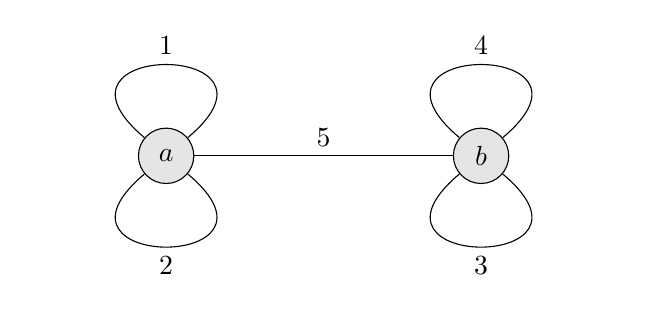
\begin{tikzpicture}
    \node[vertex] (A) at (0,0) {$a$};
    \node[vertex] (B) at (4,0) {$b$};

    % edge between vertices
    \draw (A) -- node[above] {$5$} (B);

    % loops at A
    \draw (A) to[out=140,in=40,looseness=9] node[above] {$1$} (A);
    \draw (A) to[out=220,in=320,looseness=9] node[below] {$2$} (A);

    % loops at B
    \draw (B) to[out=140,in=40,looseness=9] node[above] {$4$} (B);
    \draw (B) to[out=220,in=320,looseness=9] node[below] {$3$} (B);
\end{tikzpicture}
\]
    Here, we set $m(i)=1$ for all vertices $i=a,b$. Here, we can take the cyclic ordering as the clockwise ordering, and thus the ordering of the edges around the vertex $a$ is given by 
    $1<1<5<2<2<1$, around $b$ is given by $4<4<3<3<5<4$. The number of half-edges incident on $a$ is 5, so val($a)=5$. The same applies to $b$
    Here, we see that edge 4 is a truncated edge since $m(c)\mathrm{val}(c)=1$.
\newpage
\item[2)] Consider the following Brauer graph $G_2=(V_2,E_2,m_2,o_2)$
\par\vspace{2em}
    \begin{center}
    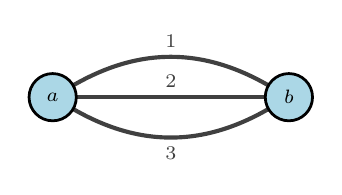
\begin{tikzpicture}
    \Vertex[x=-3,size=0.6,label=$a$]{A} \Vertex[x=0,size=0.6,label=$b$]{B}
    \Edge[bend=30,label=\;1\;,position=above](A)(B)
    \Edge[label=\;2\;,position=above](A)(B)
    \Edge[bend=30,label=\;3\;,position=below](B)(A)
    \end{tikzpicture}
    \end{center}

    We again set $m(a)=m(b)=1$ for convenience. So here, around vertex $a$, we take the clockwise ordering, which would give us the ordering\\ $1<2<3<1$ and for $b$, we can do the same which would give us $1<3<2<1$. \\
    Here, $\mathrm{val}(a)=\mathrm{val}(b)=3$ 
    \item[3)] Let us take the following graph $G_3=(V_3,E_3,m_3,o_3)$. Here the cyclic ordering around vertex $a$ is $1<2<3<1$ and at vertex $b$ is again, $1<2<3<1$, due to the nature of the edge 3.\\
    Again the valencies of both the vertices are equal to 3
    \begin{center}
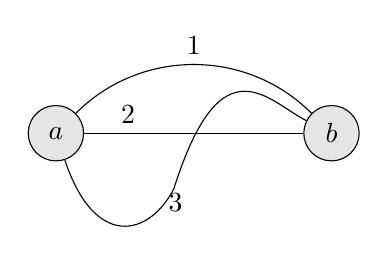
\begin{tikzpicture}

\node[vertex] (A) at (-3.5,0) {$a$};
\node[vertex] (B) at (0,0) {$b$};

\draw (A) to[bend left=45] node[above] {$1$} (B);

\draw (A) -- node[pos=0.2,above] {$2$} (B);

\draw 
(A) .. controls (-3,-1.5) and (-2.3,-1.3) .. (-2,-0.7)
     .. controls (-1.4,1.2) and (-0.8,0.4) .. 
(B)
node[pos=0.01,below] {$3$};

\end{tikzpicture}
\end{center}

\item[4)] The following example is an example of a \textit{generalised} Brauer tree, that is the underlying graph is a tree, but at least two of the vertices are of multiplicity greater than one. For example, take $G_4=(V_4,E_4,m_4,o_4)$ given by 
\begin{center}
    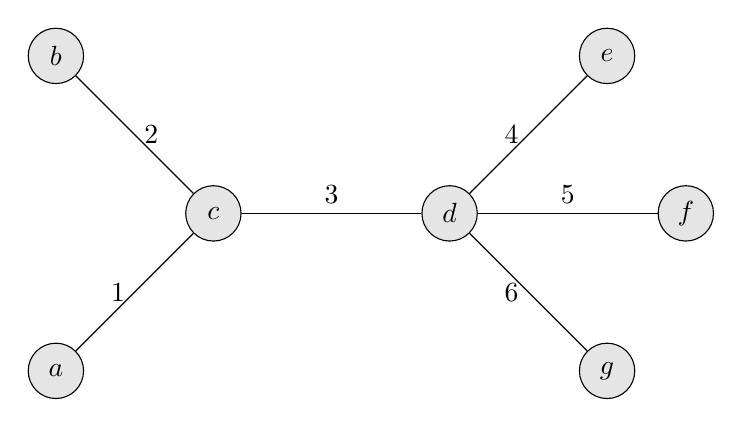
\begin{tikzpicture}
        \node[vertex] (B) at (0,0) {$b$};
        \node[vertex] (C) at (2,-2) {$c$};
        \node[vertex] (A) at (0,-4) {$a$};
        \node[vertex] (D) at (5,-2) {$d$};
        \node[vertex] (E) at (7,0) {$e$};
        \node[vertex] (F) at (8,-2) {$f$};
        \node[vertex] (G) at (7,-4) {$g$};

        \draw (B) -- node[right] {$2$} (C);
        \draw (A) -- node[left] {$1$} (C);
        \draw (C) -- node[above] {$3$} (D);
        \draw (D) -- node[left] {$4$} (E);
        \draw (D) -- node[above] {$5$} (F);
        \draw (D) -- node[left] {$6$} (G);
    \end{tikzpicture}
\end{center}

Here, we set $m(v)=1$ for all $v\in G_0$ except for $v=a,c$, and we set $m(a)=2$ and $m(c)=3$. Since $m(a)>1$, we have that the cyclic ordering of the edges around $a$ is $1<1$, around $b$ is 2 since $m(b)=1$, around $c$ is $1<2<3<1$ if we start from 1. For vertex $d$, we have $3<4<5<6<3$, for vertex $e$, we have the ordering to be 4, for vertex $f$ it is 5, and for vertex $g$ it is 6.\\
The valencies for the vertices in $G_4$ are : $\mathrm{val}(a)=\mathrm{val}(b)=\mathrm{val}(e)=\mathrm{val}(f)=\mathrm{val}(g)=1,\mathrm{val}(c)=3$ and val$(d)=4$.
\item[5)] Let us consider the following graph $G_5=(V_5,E_5,m_5,o_5)$
Again, we take the cyclic ordering in the clockwise sense. Then the ordering around $a$ is $1<3<3<2<1$, and the ordering around $b$ is $1<2<4<4<1$. The valencies are both equal, that is val$(a)=\mathrm{val}(b)=4$
\begin{center}
    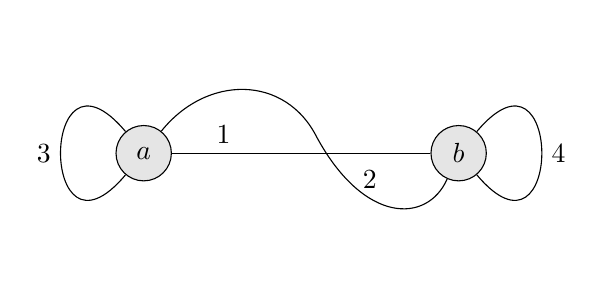
\begin{tikzpicture}

\node[vertex] (A) at (-3,0) {$a$};
\node[vertex] (B) at (1,0) {$b$};

\draw (A) -- node[pos=0.2,above] {$1$} (B);

\draw
(A)
.. controls (-2.2,1.0) and (-1.2,1.0) ..
(-0.8,0.2)
.. controls (-0.2,-0.9) and (0.6,-0.9) ..
(B)
node[pos=0.35,above] {$2$};

\draw (A) to[out=130,in=230,looseness=8] node[left] {$3$} (A);
\draw (B) to[out=50,in=310,looseness=8] node[right] {$4$} (B);
\end{tikzpicture}

\end{center}
\item[6)] 
\leavevmode
\begin{center}
    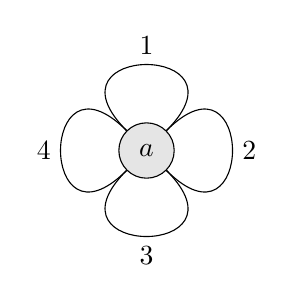
\begin{tikzpicture}
        \node[vertex] (A) at (0,0) {$a$};

\draw (A) to[out=45,in=135,looseness=8] node[above] {$1$} (A);
\draw (A) to[out=135,in=225,looseness=8] node[left] {$4$} (A);
\draw (A) to[out=225,in=315,looseness=8] node[below] {$3$} (A);
\draw (A) to[out=315,in=45,looseness=8] node[right] {$2$} (A);
    \end{tikzpicture}
\end{center}
In the above graph $G_6=(V_6,E_6,m,o)$, we again set the multiplicity of $a$ to be 1. The cyclic ordering around $a$ (clockwise) is $1<1<2<2<3<3<4<4$
\end{itemize}
\subsection{Quivers from Brauer Graphs}
In this section, we will be explaining the method on how to construct quivers from Brauer graphs, which is very powerful in the study of Brauer graph algebras.\\ 

Let $a$ be a vertex of some Brauer graph $G$, and let $i_1,i_2,...,i_n$ be the edges in $G$ incident on $a$. Here, the $e_i$'s are not necessarily distinct, that is, we might have $i_j=i_k$, for some $j,k$ if the corresponding edge is a loop. Now suppose that the cyclic ordering of these edges around $a$ is given by $i_1<i_2<...<i_n<i_1$. Then we call $i_1,i_2,...,i_n$ the \textit{successor} sequence at $a$, and we call $i_{j+1}$ the successor of $i_j$, for $1 \leq j \leq n-1$ and $i_1$ is the successor of $i_n$. Now $i_{k-1}$ is the \textit{predecessor} of $i_k$, for $2\leq k\leq n$, and $i_n$ is the predecessor of $i_1$.\\

Here, we note that if val$(v)=1$ and $m(v)>1$, then the cyclic ordering at $v$ is $e<e$ for some edge $i$, so $i$ is both the predecessor and successor of itself. But if $m(v)=1$, then the edge $i$ does not have a predecessor or successor.\\

Now, given a Brauer graph $G=(V,E,m,o)$, we define a quiver $Q_G=(Q_0,Q_1,s,t)$ in the following way:
The set of vertices $Q_0$ is given by the set of edges $E$ in $G$, where we denote the vertex $i$ in $Q_0$ by the same edge $i$ in $E$. 
In other words, if $i$ is an edge in $G$, then $i$ is a vertex in $Q$. The arrows in $Q$ are induced by the orientation $o$ in $G$.
More precisely, let $i$ and $j$ be two edges in $G$ with a common vertex $v$, such that $j$ is a direct successor of $i$ in the cyclic ordering of $v$.
Then we have an arrow $\alpha:i \to j$ in $Q_G$, and we say that $\alpha$ is given by the successor relation $(i,j)$. 
Since every arrow in $Q_G$ starts at an edge in $G$ as well as ends at an edge in $G$, therefore there are at most two arrows starting and ending at every vertex of $Q_G$, since there cannot be more than two orientations around a specific vertex $v \in V$.
Every vertex $v\in V$ such that $m(v)\mathrm{val}(v) \geq 2$, gives rise to an oriented cycle in $C_v$ in $Q_G$, since if val$(v)=1$, then $m(v)>1$, and we must have a cycle $i<i$ in $G$, for some edge $i$, or a loop in $Q_G$.
If $m(v)=1$, then val$(v)>1$, then we will have the following ordering in $G$ at the least : $i<j<i$, which will give us an oriented cycle in $Q_G$.
These cycles $C_v$ are unique up to cyclic permutation. Then, if we take $C_v$ from its cyclic permutation class such that $s(C_v)=i=t(C_v)$, then we call $C_v^i$ the \textit{special} $i$-cycle at $v$. \\

For $i  \in Q_0$, and $v \in V$, a special $i$-cycle at $v$ is not necessarily unique. However, there are at most two special $i$-cycles at $v$ for any $i \in E$, and $v \in V$, and this happens exactly when $i$ is a loop. An example of this is in Example 2.2(1). 

\textbf{Example 2.3: } In this example, we obtain the quivers from the Brauer graphs in example 2.2, and we will also list a few of the special cycles.

\begin{itemize}
    \item[1)] 
    \leavevmode
    \[\begin{tikzcd}
	&& 5 && \\
	\\
	4 &&&& 1 \\
	\\
	& 3 && 2
	\arrow["{\beta_5}"', from=1-3, to=3-1]
	\arrow["{\alpha_3}"', from=1-3, to=5-4]
	\arrow["{\beta_1}"', from=3-1, to=3-1, loop, in=170, out=100, distance=10mm]
	\arrow["{\beta_2}"', from=3-1, to=5-2]
	\arrow["{\alpha_2}"', from=3-5, to=1-3]
	\arrow["{\alpha_1}"', from=3-5, to=3-5, loop, in=80, out=10, distance=10mm]
	\arrow["{\beta_4}"', from=5-2, to=1-3]
	\arrow["{\beta_3}"', from=5-2, to=5-2, loop, in=260, out=190, distance=10mm]
	\arrow["{\alpha_5}"', from=5-4, to=3-5]
	\arrow["{\alpha_4}"', from=5-4, to=5-4, loop, in=350, out=280, distance=10mm]
\end{tikzcd}\]

Special cycles in $Q_{G_1}$ are the special 1-cycles at $a$ corresponding to $\alpha_1\alpha_2\alpha_3\alpha_4\alpha_5$ and $\alpha_2\alpha_3\alpha_4\alpha_5\alpha_1$.\\
The special 2-cycles at $a$ are given by $\alpha_2\alpha_3\alpha_0\alpha_1$.\\
The special 3-cycle at $a$ is given by $\alpha_3\alpha_0\alpha_1\alpha_2$.\\
The special 2-cycle at $b$ is given by $\beta_1\beta_2\beta_3$.\\
The special 4-cycle at $b$ is given by $\beta_2\beta_3\beta_1$.\\
The special 3-cycle at $b$ is $\beta_3\beta_1\beta_2$

    \item[2)] 
    \leavevmode
    \begin{center}
        \[\begin{tikzcd}[row sep=huge,column sep=huge]
	& 1 & \\
	\\
	3 && 2
	\arrow["{\beta_1}", shift left, from=1-2, to=3-1]
	\arrow["{\alpha_1}", shift left, from=1-2, to=3-3]
	\arrow["{\alpha_3}", shift left, from=3-1, to=1-2]
	\arrow["{\beta_2}", shift left, from=3-1, to=3-3]
	\arrow["{\beta_3}", shift left, from=3-3, to=1-2]
	\arrow["{\alpha_2}", shift left, from=3-3, to=3-1]
\end{tikzcd}\]
    \end{center}
The special 1-cycle at $a$ is given by $\alpha_1\alpha_2\alpha_3$.\\
The special 2-cycle at $a$ is given by $\alpha_2\alpha_3\alpha_1$.\\
The special 3-cycle at $a$ is given by $\alpha_3\alpha_1\alpha_2$.\\
The special 1-cycle at $b$ is given by $\beta_1\beta_2\beta_3$.\\
The special 2-cycle at $b$ is given by $\beta_3\beta_1\beta_2$.\\
The special 3-cycle at $b$ is given by $\beta_2\beta_3\beta_1$.\\

\item[3)] 

\leavevmode
\begin{center}
\[\begin{tikzcd}[row sep=huge,column sep=huge]
	& 1 & \\
	\\
	3 && 2
	\arrow["{\alpha_1}", shift left, from=1-2, to=3-3]
	\arrow["{\beta_1}"', shift right, from=1-2, to=3-3]
	\arrow["{\alpha_3}", shift left, from=3-1, to=1-2]
	\arrow["{\beta_3}"', shift right, from=3-1, to=1-2]
	\arrow["{\alpha_2}", shift left, from=3-3, to=3-1]
	\arrow["{\beta_2}"', shift right, from=3-3, to=3-1]
\end{tikzcd}\]
\end{center}
The special 1-cycle at $a$ is given by $\alpha_1\alpha_2\alpha_3$\\
The special 2-cycle at $a$ is given by $\alpha_2\alpha_3\alpha_1$\\
The special 3-cycle at $a$ is given by $\alpha_3\alpha_1\alpha_2$\\
The special 1-cycle at $b$ is given by $\beta_1\beta_2\beta_3$\\
The special 2-cycle at $b$ is given by $\beta_2\beta_3\beta_1$\\
The special 3-cycle at $b$ is given by $\beta_3\beta_1\beta_2$\\

    \item[(4)]
    \leavevmode
    \begin{center}
        \[\begin{tikzcd}[row sep=huge,column sep=huge]
	2 && 4 & \\
	& 3 && 5 \\
	1 && 6
	\arrow["{\alpha_2}", from=1-1, to=2-2]
	\arrow["{\beta_2}", from=1-3, to=2-4]
	\arrow["{\beta_1}", from=2-2, to=1-3]
	\arrow["{\alpha_3}", from=2-2, to=3-1]
	\arrow["{\beta_3}", from=2-4, to=3-3]
	\arrow["{\alpha_1}", from=3-1, to=1-1]
	\arrow["{\beta_4}", from=3-3, to=2-2]
   \arrow["\rho", out=310, in=230, distance=2.5em, from=3-1, to=3-1]
\end{tikzcd}\]
    \end{center}
    The special cycles in $Q_{G_4}$ are as follows : 

\begin{itemize}
    \item[$C_c^1$: ] $\alpha_1\alpha_2\alpha_3$ 
    \item[$C_c^2$: ] $\alpha_2\alpha_3\alpha_1$ 
    \item[$C_c^3$: ] $\alpha_3\alpha_1\alpha_2$ 
    \item[$C_d^3: $] $\beta_1\beta_2\beta_3\beta_4$
\end{itemize}
\item[5)] 
\leavevmode
\begin{center}
    \[\begin{tikzcd}[sep=large]
	& 1 & \\
	4 && 3 \\
	& 2
	\arrow["{\alpha_1}", from=1-2, to=2-3]
	\arrow["{\beta_1}"', shift right, from=1-2, to=3-2]
	\arrow["{\beta_4}", from=2-1, to=1-2]
	\arrow["{\beta_3}", from=2-1, to=2-1, loop, in=145, out=215, distance=10mm]
	\arrow["{\alpha_2}", from=2-3, to=2-3, loop, in=325, out=35, distance=10mm]
	\arrow["{\alpha_3}", from=2-3, to=3-2]
	\arrow["{\alpha_4}"', shift right, from=3-2, to=1-2]
	\arrow["{\beta_2}", from=3-2, to=2-1]
\end{tikzcd}\]
\end{center}
This is similar to 1), but there is a loop on both sides now. The special 1-cycle at $a$ is given by $\alpha_1\alpha_2\alpha_3\alpha_4$.\\
The special 3-cycles at $a$ are given by $\alpha_2\alpha_3\alpha_4\alpha_1$ and $\alpha_3\alpha_4\alpha_1\alpha_3$.\\
The special 2-cycle at $a$ is given by $\alpha_4\alpha_1\alpha_2\alpha_3$.\\
The special 1-cycle at $b$ is given by $\beta_1\beta_2\beta_3\beta_4$\\
The special 4-cycles at $b$ are given by $\beta_3\beta_4\beta_1\beta_2$ and $\beta_4\beta_1\beta_2\beta_3$.\\
The special 2-cycle at $b$ is given by $\beta_2\beta_3\beta_4\beta_1$.
\item[6) ]
\leavevmode
\[\begin{tikzcd}
	&& 1 && \\
	\\
	4 &&&& 2 \\
	\\
	&& 3
	\arrow["{\alpha_8}", from=1-3, to=1-3, loop, in=55, out=125, distance=10mm]
	\arrow["{\alpha_1}", from=1-3, to=3-5]
	\arrow["{\alpha_7}", from=3-1, to=1-3]
	\arrow["{\alpha_6}", from=3-1, to=3-1, loop, in=145, out=215, distance=10mm]
	\arrow["{\alpha_2}", from=3-5, to=3-5, loop, in=325, out=35, distance=10mm]
	\arrow["{\alpha_3}", from=3-5, to=5-3]
	\arrow["{\alpha_5}", from=5-3, to=3-1]
	\arrow["{\alpha_4}", from=5-3, to=5-3, loop, in=235, out=305, distance=10mm]
\end{tikzcd}\]
Again, we have loops at all the vertices in the quiver, and so we have two special $i$-cycles at each vertex.
The special cycles in $Q_{G_6}$ are 
\begin{itemize}
    \item Corresponding to 1, we have $\alpha_8\alpha_1\alpha_2\alpha_3\alpha_4\alpha_5\alpha_6\alpha_7$ and $\alpha_1\alpha_2\alpha_3\alpha_4\alpha_5\alpha_6\alpha_7\alpha_8$
    \item Corresponding to 2, we have $\alpha_2\alpha_3\alpha_4\alpha_5\alpha_6\alpha_7\alpha_8\alpha_1$ and $\alpha_3\alpha_4\alpha_5\alpha_6\alpha_7\alpha_8\alpha_1\alpha_2$
    \item Corresponding to 3, we have $\alpha_4\alpha_5\alpha_6\alpha_7\alpha_8\alpha_1\alpha_2\alpha_3$ and $\alpha_5\alpha_6\alpha_7\alpha_8\alpha_1\alpha_2\alpha_3\alpha_4$
    \item Corresponding to 4 , we have $\alpha_6\alpha_7\alpha_8\alpha_1\alpha_2\alpha_3\alpha_4\alpha_5$ and $\alpha_7\alpha_8\alpha_1\alpha_2\alpha_3\alpha_4\alpha_5\alpha_6$
\end{itemize}
\end{itemize}
\newpage
\subsection{Set of relations and definition of Brauer graph algebras}
Here, we define what is called an ideal of relations $I_G$ in $KQ_G$, the path algebra of $Q_G$. This ideal is generated by three types of relations. For this we recall that we identify the set of edges $E$ of a Brauer graph $G$ with the set of vertices $Q_0$ of the corresponding quiver $Q_G$ and that we denote the set of vertices of the Brauer Graph by $V$. Also, when we say relation, we mean 

\textit{Relations of type I:}
\[
C_v^i - C_{v'}^i,
\]
for any $i\in Q_0$ and for any two distinct special $i$-cycles $C_v^i$ and $C_{v'}^i$ such that both $v$ and $v'$ are not truncated. In other words, $m(v)\mathrm{val}(v)\neq1$ and $m(v')\mathrm{val}(v')\neq 1$.

\textit{Relations of type II}:
\[
C_v^i\alpha_1
\] for any $i\in Q_0$ and any $v\in V$ and where $C_v^i$ is any special $i$-cycle $C_v=\alpha_1\alpha_2...\alpha_n$.

\textit{Relations of type III: }
\[
\alpha\beta
\]

for any $\alpha,\beta \in Q_1$ such that $\alpha\beta$ is not a subpath of any special cycle except if $\alpha=\beta$ is a loop associated to a vertex $v$ of valency one and multiplicity $m(v)>1$.\\

The algebra $A_G=KQ_G/I_G$ is called the \textit{Brauer graph algebra} associated to the Brauer graph $G$

\textbf{Examples 2.4: } Sets of relations for the examples in 2.2
\begin{itemize}
    \item Set of the three types of relations defining the Brauer graph algebra $B_1=KQ_G{_1}/I_{G_1}$:
    
\end{itemize}







\end{document}